\section{Introduction}

The generation of high-quality educational explanations represents a fundamental challenge in natural language processing. Unlike general-purpose conversational tasks, educational rationales must simultaneously satisfy two competing requirements: they must be \textit{logically grounded}---deriving the correct answer through sound deductive steps---and \textit{linguistically fluent}---maintaining natural, readable prose appropriate for a learner audience.

Supervised Fine-Tuning (SFT) on teacher-generated demonstrations has become the standard approach to instilling this capability into LLMs. However, SFT models exhibit a consistent and critical failure mode: while they produce fluent, confident-sounding text, they rarely construct the deductive chain that justifies \textit{why} the correct answer follows from the question context. Empirically, SFT models in our study achieve NLI entailment scores of only 0.05--0.22, indicating that the generated explanation rarely logically implies the ground-truth answer---even when the model ``knows'' the fact.

Reinforcement Learning from Human Feedback (RLHF) and its efficient derivative, Direct Preference Optimization (DPO) \cite{rafailov2023direct}, have sought to move beyond SFT by aligning models to human preferences. Yet these approaches contain a structural flaw when applied to factually demanding tasks: \textbf{the preference signal does not measure logical correctness}. Human annotators---and LLM judges---exhibit a well-documented \textit{verbosity bias}, systematically preferring longer, rhetorically polished responses over concise, logically precise ones \cite{zheng2023judging}. As we demonstrate empirically, GPT-4o-mini awards a 69\% win rate to a verbose SFT baseline over a more logically precise but concise RL-aligned model. DPO trained on such signals therefore reinforces stylistic fluency at the expense of factual grounding, leaving the core alignment gap unaddressed.

A natural remedy is to replace human preference labels with an automated logical metric---specifically, NLI entailment probability. However, optimizing DPO solely against NLI entailment incurs what we term the \textbf{alignment tax}: the model learns to produce short, repetitive snippets that satisfy the NLI scorer but collapse in linguistic coherence. This trade-off between logical soundness and readability represents a fundamental tension that single-dimensional reward signals cannot resolve.

\begin{figure}[h]
\centering
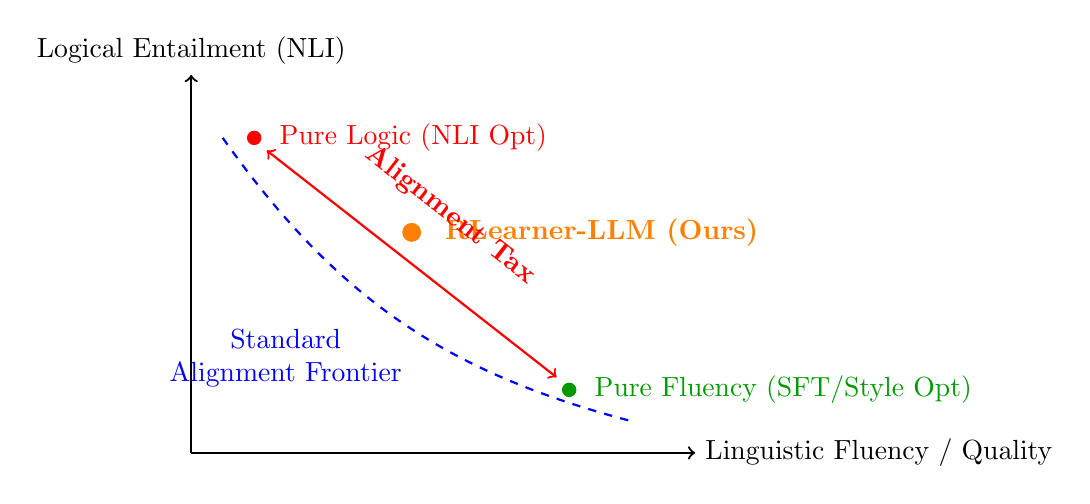
\begin{tikzpicture}[scale=0.8]
% Axes
\draw[->, thick] (0,0) -- (8,0) node[right] {Linguistic Fluency / Quality};
\draw[->, thick] (0,0) -- (0,6) node[above] {Logical Entailment (NLI)};

% Curves
\draw[blue, thick, dashed] (0.5,5) to[bend right=20] (7,0.5);
\node[blue, align=center] at (1.5,1.5) {Standard\\Alignment Frontier};

% Points
\filldraw[red] (1,5) circle (3pt) node[right=0.2cm] {Pure Logic (NLI Opt)};
\filldraw[green!60!black] (6,1) circle (3pt) node[right=0.2cm] {Pure Fluency (SFT/Style Opt)};
\filldraw[orange] (3.5,3.5) circle (4pt) node[right=0.3cm] {\textbf{RLearner-LLM (Ours)}};

% Annotations
\draw[<->, red, thick] (1.2,4.8) -- (5.8,1.2) node[midway, sloped, above=0.5cm] {\textbf{Alignment Tax}};

\end{tikzpicture}
\caption{Conceptual illustration of the \textbf{Alignment Tax}. Standard optimization forces a trade-off between logical grounding and linguistic fluency. RLearner-LLM pushes the Pareto frontier toward the upper-right quadrant through a dual-signal hybrid reward.}
\label{fig:alignment_tax}
\end{figure}

In this paper, we propose \textbf{RLearner-LLM}, a framework that resolves this tension by addressing the root cause directly: the reward signal used to construct preference pairs. Our key insight is that logical grounding and linguistic fluency are \textit{complementary objectives}, not competing ones---and that an automated dual-signal reward combining NLI entailment (for logical soundness) with a verifier score (for pedagogical quality) can construct high-fidelity preference pairs without human annotation, while simultaneously avoiding the degenerate solutions that plague single-signal optimization.

Our contributions are as follows:
\begin{enumerate}
    \item \textbf{Problem diagnosis}: We identify that the root cause of logical misalignment in DPO-trained educational models is not the optimization algorithm itself, but the \textit{reward signal blindspot}---the inability of standard preference signals to measure logical correctness. We provide empirical evidence of verbosity bias in LLM-as-a-judge evaluation that perpetuates this blindspot.
    \item \textbf{Hybrid-DPO framework}: We introduce \textbf{RLearner-LLM}, which automatically constructs preference pairs $\mathcal{D}_{pref}$ using a composite score $H(E_i) = 0.5 \cdot P_{NLI} + 0.5 \cdot S_{Verifier}$, fusing a DeBERTa-v3 NLI signal with a verifier LLM score. This eliminates the need for human annotation while overcoming the alignment tax.
    \item \textbf{Cross-architecture validation}: We validate across two architectures (LLaMA-2-13B, Qwen3-8B) and five academic domains (Biology, Medicine, Law), demonstrating up to 6$\times$ NLI improvement over SFT baselines and consistent ACR gains even on stronger base models, achieving a 95\% GPT-4o-mini win rate.
\end{enumerate}
